%!TEX root = vis4_report.tex
\section{Grasping}
\autsubsection{Motivation}{Malthe Høj-Sunesen}
Humans spend years learning how to grasp objects.
Babies have a hard time figuring out how to grasp even the most simple objects,
and parents solve that problem by giving babies and children plastic cutlery, bouncy, soft toys and always walking around with an eye on each finger.
We come to expect of a child to drop toys, knock over glasses, and the like.

A robot is not allowed to fail in the same way.
When a robot's hand grasps something we expect it to not let it go --- or worse, drop it --- before it is supposed to.
In a tightly controlled production line that is not a problem.
Using embodied AI the parts can be aligned perfectly for the robot and the robot can assemble the parts correctly.

In a not so tightly controlled environment among people it is a bigger problem.
If a service robot is supposed to clean up mess left after a human, it is almost guaranteed that the parts are not aligned as a robot could predict.
If an industrial robot can figure out the best grasp autonomously for an object it would decrease operator dependency,
leading to faster setup and lower costs for the company.

\autsubsection{Simplifying objects to primitive models}{Malthe Høj-Sunesen}\label{ssec:millergrasp}
Biederman suggested that elements can be broken down to geons, basic elements describing one feature of an object.

\begin{figure}
	\centering
	%Trim: Left, lower, right, upper
	\includegraphics[page=3, trim=2.5cm 21.2cm 11.5cm 3.2cm, clip]{MillerEtAl}
	\caption{``A mug and its primitive representation''; a cylinder and a box. From~\cite{miller}.}
\label{fig:miller3}
\end{figure}

In~\cite{miller} the idea behind geons is used to help a robot simulator find good grasps.
The robot knows how to grasp each shape primitive (equivalent to geon).
Any object is then reduced to its shape primitives where applicable.
This allows a simulator to know which points are good to grasp, resulting in simpler calculations.
An example of this reduction can be seen in Figure~\ref{fig:miller3} with shape primitive building bricks shown in Figure~\ref{fig:miller4}.

\begin{figure}
	\centering
	\includegraphics[page=3, trim=11.5cm 17.2cm 2.6cm 3.2cm, clip]{MillerEtAl}
	\caption{``Examples for grasp generation on single primitives.
    The balls represent starting positions for the center of the palm.
    A long arrow shows the grasp approach direction, and a short arrow shows the thumb direction.
    In most grasp locations, two or more grasp possibilities are shown, each with a different thumb direction.'' From~\cite{miller}.}
\label{fig:miller4}
\end{figure}

Reducing the visual information in this way will give the simulator a simpler task,
as it does not have to simulate thousands of possible grasps but only the grasps based on the preshape grasps per primitive representation.
An example of the found grasps can be seen in Figure~\ref{fig:miller6}.

\begin{figure}
	\centering
	\includegraphics[page=6, angle=270, trim=2.1cm 2.1cm 15.7cm 14.3cm, clip]{MillerEtAl}
	\caption{The primitive mug representation and the two best grasps. The red cones indicate point-of-contact. From~\cite{miller}.}
\label{fig:miller6}.
\end{figure}

\autsubsection{Learning to grasp through attempts}{Malthe Høj-Sunesen}
Much like~\cite{miller} in Section~\ref{ssec:millergrasp} tried to emulate how the human vision works according to Biederman,
so do~\cite{detry} try to emulate how a child learns to grasp objects.
Any parent will tell you that their child did not quite know how to actively grasp\footnote{Let alone letting it go again!} toys from the beginning.
Where to hold is one of the problems.

The approach in~\cite{detry} is to let a robotic platform learn how to grasp a single object. 
Using stereo vision, the 3D features of an object can be calculated.
The system will then try to calculate where that object can be picked up.
An example of where the system calculates a toy pan can be grasped can be seen in Figure~\vref{fig:detry11}. s

\begin{figure}
	\centering
	\includegraphics[page=23, angle=90, trim=3.2cm 8.7cm 12cm 11.5cm, clip]{DetryEtAl}
	\caption{Left: A full graph of the possible grasp positions.
		Right: Clearer showing of what the sticks mean;
		the stick is the robotic hand's translation while the paddle at the end is the point where the fingers close. From~\cite{detry}}
	\label{fig:detry11}
\end{figure}

After calculating where the object can be grasped, the robot will start to grasp the object, time and time again. 
In~\cite{detry}, the robot performed more than 2000 grasps.
During the grasp trials the robot and vision system will see if the grasp is stable, ie.\ if the object is not moving. 
Using all the trials the robot system can build a model of the possibility that a grasp will be successful. 
The result is visualized in Figure~\vref{fig:detry4}.

\begin{figure}
	\centering
	\includegraphics[page=11, trim=4.5cm 17cm 4.5cm 5.5cm, clip]{DetryEtAl}
	\caption{``Various projections of a grasp density generated by a robot''. The greener the pixel, the higher the density and thus probability of a good grasp. From~\cite{detry}.}
\label{fig:detry4}
\end{figure}

In the end, the robot has learned how to pick up an object from any angle,
and is able to choose the best possible grasp in any situation.
This is indeed how children and grown-ups know how to pick up objects as well.

\autsubsection{Elementary grasping actions}{Hsin-Yu Lee}
The Elementary Grasping Actions, which also called EGA, is the specific grasping gestures used in the paper~\cite{kootstra} that was implemented once after we find the object by the ECV system. 
The EGA was also mentioned and defined in the paper~\cite{pugeault}. 
The Figure~\vref{fig:kootstra1} shows the three different ways of grasping object base on edge and surface information separately. 
Basically, the directions, approaching ways and positions are pre-defined, only slightly changed according to the size of the surface or the distance between two selected contours. 

We can simply choose one method to grasp something; we also can use the simulator to help us select the best grasping action through these methods. There are several experiments presented in the paper~\cite{kootstra} shows the performance of each different actions and in the circumstance of using multiple method at the same time. 

\begin{figure}
	\centering
	\includegraphics[width=1\textwidth, page=2, trim=1.6cm 19.1cm 1.6cm 3cm, clip]{KootstraEtAl}
	\caption{The elementary grasping actions (EGA) are illustrated on the top with some examples of real grasps on the bottom. (a-c) The three contour-based EGAs. The red lines indicate the selected contours. (d-f) The surface-based EGAs. The dark faces show the selected surface. The first letter in the naming scheme marks the type of features used to generate a grasp. ’c’ stands for contour and ’s’ for surface. The first subscript stands for two or three fingers. The last subscript marks the general type of grasp, where ’1’ is an encompassing grasp, ’2’ is a pinch grasp from the top and ’3’ is a pinch grasp from the side of the surface. For each type of grasping action, an example is shown consisting of an original image, a snapshot of the ECV representation along with the selected grasp, and the grasp execution in the simulation/real setup. From~\cite{kootstra}}
	\label{fig:kootstra1}
\end{figure}